\documentclass[../../Aurora C# unofficial manual.tex]{subfiles}

\begin{document}
	\section{Formation templates}
	Original post can be found
	\href{http://aurora2.pentarch.org/index.php?topic=8495.msg105832#msg105832}{here}.
	\\\\
	
	The screenshot below shows the Formation Templates tab of the Ground Forces window. Formation Templates are the equivalent of VB6 Ground Unit Types, although it might be easier to think of them as serving the same function as Ship Classes. They are a detailed design that serves as a template for building Formations based on that same design, which is the same relationship as Ship Classes to Ships.
	
	This tab is split into two halves. On the left is a list of available Ground Unit Classes created using the Unit Class Design tab (as explained in the previous rules post). All of these were created using TL4 technology, with three exceptions. For comparison purposes, the Challenger 2 Main Battle Tank and the Warrior AFV were created using Conventional, rather than Trans-Newtonian, technology, while the Challenger Base TN Upgrade was the Challenger design with TL1 technology. It should be possible to simulate most modern army units with the new C\# Aurora ground combat, so you could theoretically be landing on an alien world with Abrams and Bradleys or T-14 and T-15 Armatas. The ten columns for the Unit Class List are as follows:
	\begin{enumerate}
		\item Type: An abbreviation for the Base Type (infantry, Vehicle, Heavy Vehicle, etc.)
		\item Name: The name assigned during Unit Class Design. This can be changed using the Rename Unit button.
		\item Size: Transport size in tons.
		\item Cost: Cost in Build Points.
		\item Arm: The Armour Strength of the Unit. This is based on the armour available at the time of design and is not upgraded when newer technology becomes available (as with ship designs).
		\item HP: The Hit Points of the Unit. This is set at design time and does not change.
		\item Components A to D: Abbreviations for each of the components included in the Unit Class. These are the same abbreviations as used on the Components table in the Unit Class Design tab. As with armour and hit points, any components use the technology available at the time of unit design. To see the detailed view of the components, click on the Unit. The Unit Summary will be shown in the bottom section on the left hand side.
	\end{enumerate} 
	
	As an example, the Leman Russ Battle Tank is a Heavy Vehicle of 104 tons, with 60 Armour and 60 Hit points, costing 12.48 BP. The components are Heavy Anti-Vehicle (HAV) and Heavy Crew-Served Anti-Personnel (HCAP). Looking at the summary, the HAV has 1 shot per combat phase with Penetration 60 and Damage 60, while the HCAP has 6 shots with Penetration 20 and Damage 10.
	
	The right-hand half of the tab shows Formation Templates. A new Formation Template is created by clicking the New button. In this case, four have already been created. Each Template comprises one or more Template Elements, shown in the bottom right section Each Template Element has a specific number of specific Ground Unit Class. For example, the Guard Armoured Regiment is currently selected, which has four template elements: 60x Leman Russ Battle Tank, 1x Macharius Command Tank, 12x Hydra Flak Tank and 24x Hellhound Anti-Infantry Tank.
	
	Each template element has the following attributes:
	\begin{enumerate}
		\item Name: The Unit Class for this element.
		\item Units: The number of units of that Unit Class in this element.
		\item Size: The total size on tons of this element. For example, 60 Leman Russ Battle Tanks at 104 tons each is 6,240 tons.
		\item Cost: The total cost in Build Points for this element.
		\item HP: The total aggregate hit points for the element.
		\item HQ: The headquarters capacity of the elements Unit Class in tons. If there are multiple units in a template element, only one is considered for the headquarters capacity. Any additional units are for redundancy. The headquarters capacity is the total size of the formation (or formation hierarchy) that can be effectively controlled by a commander based in a unit with this component. In the case of the Macharius Command Tank, it has an HQ capacity of 10,000 tons.
		\item FFD: The total number of Forward Fire Direction (FFD) components in the template element. Forward Fire Direction allows a front-line unit to direct the fire of bombardment units from a formation in a support position, fighters on close air support missions, or ships in orbit.
		\item Const. The construction value of the element in Construction Factory Equivalents (CFEs).
		\item CIWS: The number of Close-in-Weapon-System components in the template element, capable of defending the planet (on which the unit is based) from missile attack.
		\item STO: The number of Surface-To-Orbit energy weapon components in the template element. STOs are capable of engaging ships in space within weapon range of the planet on which the unit is based.
	\end{enumerate} 
	
	The totals for each Template Element are added together to create the total for the Formation Template as a whole, shown in the top right section. In the example shown, the Guard Armoured Regiment has a total size of 8,942 tons, which is the combination of all four template elements. The Formation Template list has an additional column for Rank. A default rank will be suggested by the program, although this can be overridden by the player. This rank will be used by Automated Assignment process for any Formations built using this Formation Template.
	
	To add new Template Elements to a Formation Template, use the Add Units button in conjunction with the adjacent text field to specify the number of units in the new element. This number can be subsequently edited by selecting the element and clicking the Edit Amount button. Both Formation Templates and Element Templates can be deleted using the appropriate buttons.
	
	This screenshot shows the Macharius Command Tank on the left and the Brigade Headquarters formation template on the right. The Macharius is a super-heavy vehicle, with two super-heavy anti-vehicle weapons and an HQ4 component, which provides a headquarters capacity of 10,000 tons. This is a large and expensive vehicle at 518 tons and 93.24 BP, but is well-protected as the loss of the HQ in a formation will result in the loss of any commander bonuses (and maybe the commander himself).
	\begin{figure}[H]
		\centering
		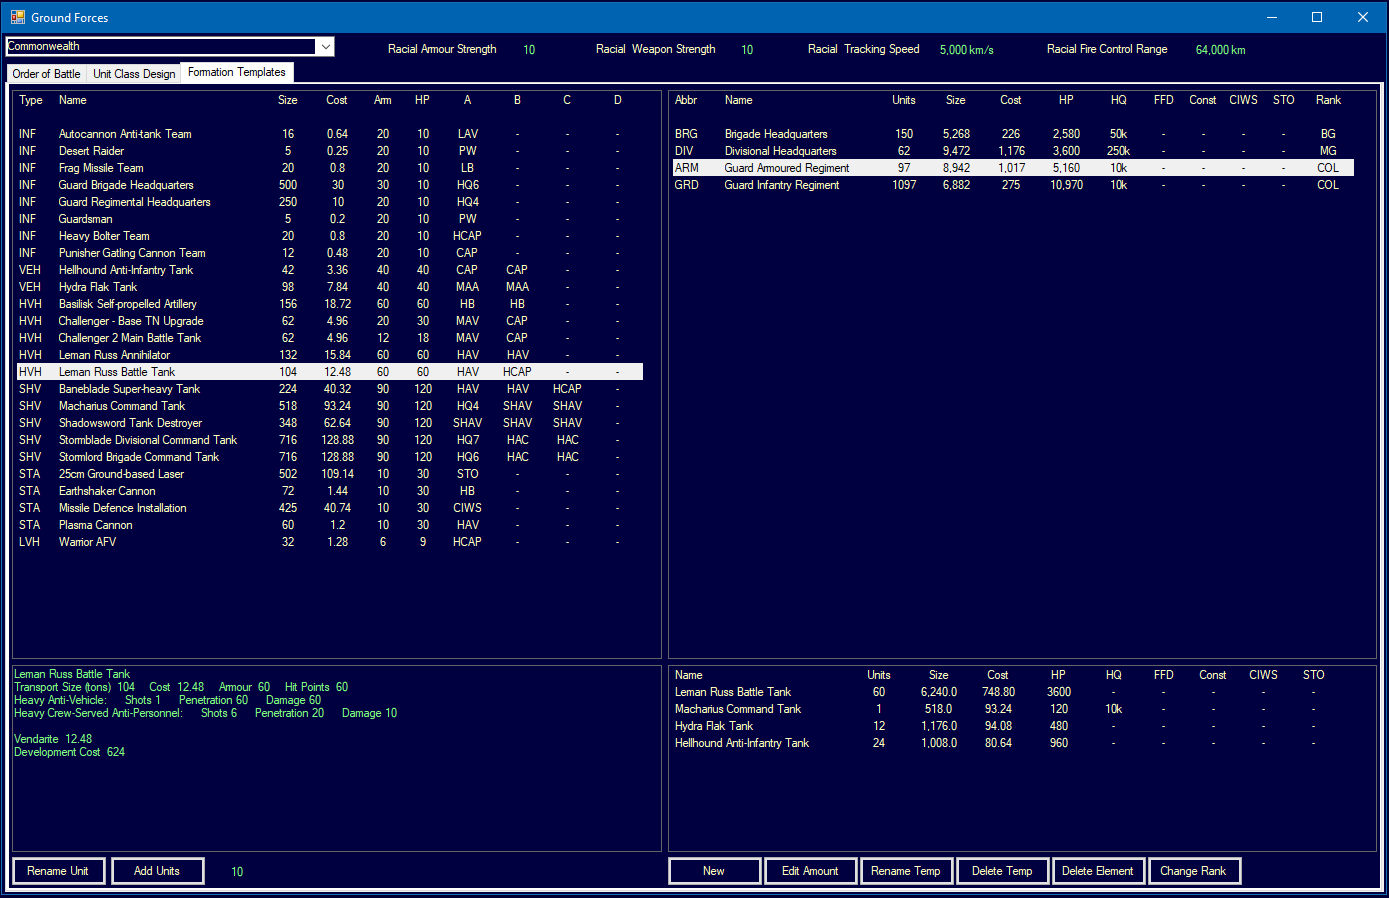
\includegraphics[width=0.95\linewidth]{images/FormationTemplates}
		\caption[Formation Templates]{Formation Templates Example 1}
		\label{fig:formationtemplates}
	\end{figure}
	
	The Brigade Headquarters formation template includes two Guard Brigade Headquarters units, in case one is destroyed, plus thirty-six large artillery pieces, twelve flak tanks and a company of Guardsman. Combat involves three locations. Front-Line, Support or Rear-Echelon. Units in a Support position can only attack using bombardment weapons, or defend themselves against air attack. This formation is intended to serve in the Support location and is organising accordingly. However, it is possible for a Support Formation to temporarily find itself moved into a Front-Line position, so the Guardsman Element will provide additional protection in that case.
	\begin{figure}[H]
		\centering
		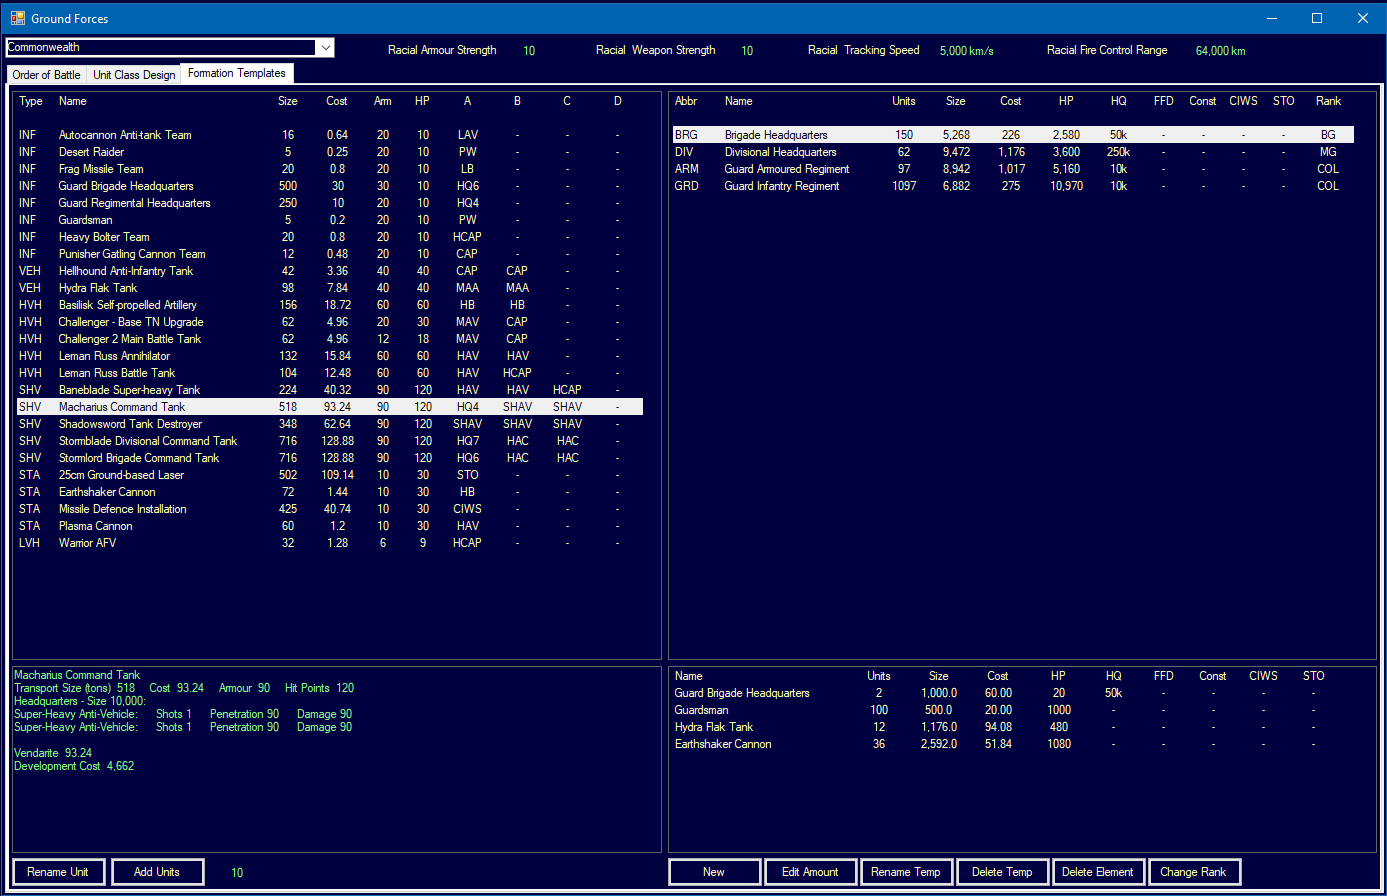
\includegraphics[width=0.95\linewidth]{images/FormationTemplates2}
		\caption[Formation Templates]{Formation Templates Example 2}
		\label{fig:formationtemplates2}
	\end{figure}
\end{document}